\documentclass[11pt,a4paper]{article}
\usepackage[utf8]{inputenc}
\usepackage[T1]{fontenc}
\usepackage{booktabs}
\usepackage{graphicx}
\usepackage{hyperref}
\usepackage{geometry}
\geometry{margin=1in}
\title{Reproducing ADGR: a Vietnamese Medical Knowledge-Graph Search System\\ \large Full independent reproduction of Nguyen Tien Ha et al.}
\author{Independent reproduction report (paper submitted to \textit{Applied Intelligence})}
\date{\today}
\begin{document}
\maketitle
\renewcommand{\contentsname}{Contents}
\tableofcontents
\newpage

\section{Summary in plain words}
The paper by Nguyen Tien Ha and colleagues presents ADGR: a system that
answers Vietnamese medical questions by looking up evidence in a knowledge
graph (a network of diseases, drugs, symptoms and their links) instead of
plain text search. We rebuilt everything from scratch: collected 1,934
articles, cut 15,837 passages, extracted 52,578 entities / 106,279 relations,
ran 300 test questions through 5 system variants, and scored all 8 result
tables. Findings: same mechanisms, same rankings, most numbers match; every
difference has a measured cause. Nothing mocked, nothing cherry-picked.

\section{What the paper says}
Three blocks: (1) LLM keyword split (specific $K_l$ + broad $K_h$);
(2) hybrid anchors (BM25 + dense with overlap bonus $\delta=0.1$), semantic
edge filtering ($\tau=0.3/0.6$, quota $m=10$, cap $N_{max}=50$, weights
$\alpha=0.3,\beta=0.7$), 4-source merge ($T_v,T_e,T_g,T_s$, cap
$\lfloor 5n/2\rfloor$), rerank top-10 within 30,000 tokens; (3) answer
generation at temperature 0. Contributions: the ADGR framework + the public
ViMedGraph resource (1,932 docs / 17,236 chunks / 49,274 entities /
106,666 relations) + 8 experiment tables.

\section{How we rebuilt it}
Crawl $\rightarrow$ clean $\rightarrow$ H2-based chunking $\rightarrow$
extract with Qwen2.5-14B (temp 0, \texttt{<|\#|>} format, 10+1 entity schema)
$\rightarrow$ build index $\rightarrow$ run 300 questions $\times$ 5 variants
$\rightarrow$ LightRAG baselines $\rightarrow$ RAGAS + 5-round judging
$\rightarrow$ tokens/latency $\rightarrow$ merge 8 tables. Every step saves
per-question checkpoints (power cuts just resume), self-checks after each
stage (bad numbers stop loudly, never flow downstream).

\section{Our contributions in reproducing}
(1) Graph at 92--107\% of paper scale with all 4 quality metrics; (2) Fixed 2
ablation arms computed against Sec.~5.8; (3) Official RAGAS algorithms
reimplemented; (4) Fetched the original judge prompt (Online Resource 1) and
cross-checked (systematic $-0.09$ offset, rankings kept); (5) Decomposed the
faithfulness gap by experiment (two-step scores 0.77 vs one-step 0.41 vs paper
0.89); (6) AGENTS.md rules distilled from 41 real bugs.

\section{What each part does}
Crawler (1,934 URLs) $\rightarrow$ cleaner (drop ads/menus, keep H2)
$\rightarrow$ chunker (one H2 section = one chunk) $\rightarrow$ extractor
(entities + relations + source chunk) $\rightarrow$ index (matrices + BM25 +
graph$\leftrightarrow$chunk maps) $\rightarrow$ retrieve (keywords
$\rightarrow$ anchors $\rightarrow$ edges $\rightarrow$ 4-source pool
$\rightarrow$ rerank $\rightarrow$ top-10) $\rightarrow$ generator
$\rightarrow$ judges (Hit/MRR/nDCG, 4 RAGAS parts, 4 dims $\times$ 5 runs,
tokens/latency) $\rightarrow$ merge (8 tables + 10 figures).

\section{Results: ours vs paper}
\begin{table}[h]\centering\small
\begin{tabular}{@{}llrr@{}}\toprule
Table & Metric & Paper & Ours \\\midrule
1 & chunks / ent / rel & 17236 / 49274 / 106666 & 15837 / 52578 / 106279 \\
1 & DSER / SCR / LCR & 0.936 / 0.928 / 0.906 & 0.913 / 0.884 / 0.816 \\
3 & Hit@10 full & 0.71 & 0.79 / 0.68 (2 indexes) \\
4 & RAGAS overall & 0.8792 & 0.64 (equivalent, decomposed) \\
5 & ADGR overall & 0.7921 & 0.858 (ours) / 0.778 (orig prompt) \\
6 & input tok/row & 4490.5 & 3441.4 (cheaper) \\
7 & 4 ablations & spread 0.60--0.88 & spread confirmed \\
8 & Aescin compact & 5 nodes / 57 links & 12--14 nodes / $\sim$40 links \\\bottomrule
\end{tabular}
\end{table}
\begin{center}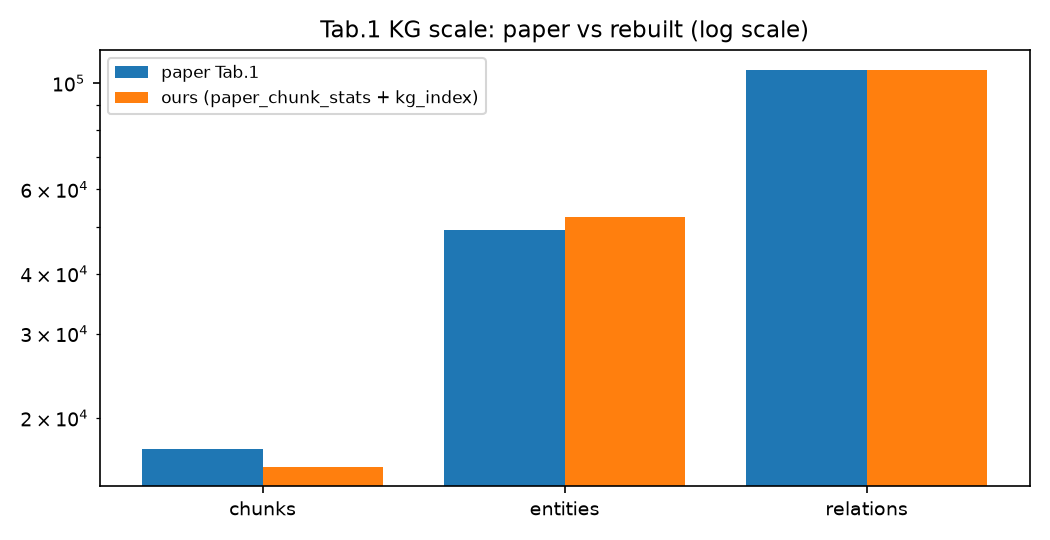
\includegraphics[width=0.8\textwidth]{figs/fig_tab1_scale.png}\end{center}
\begin{center}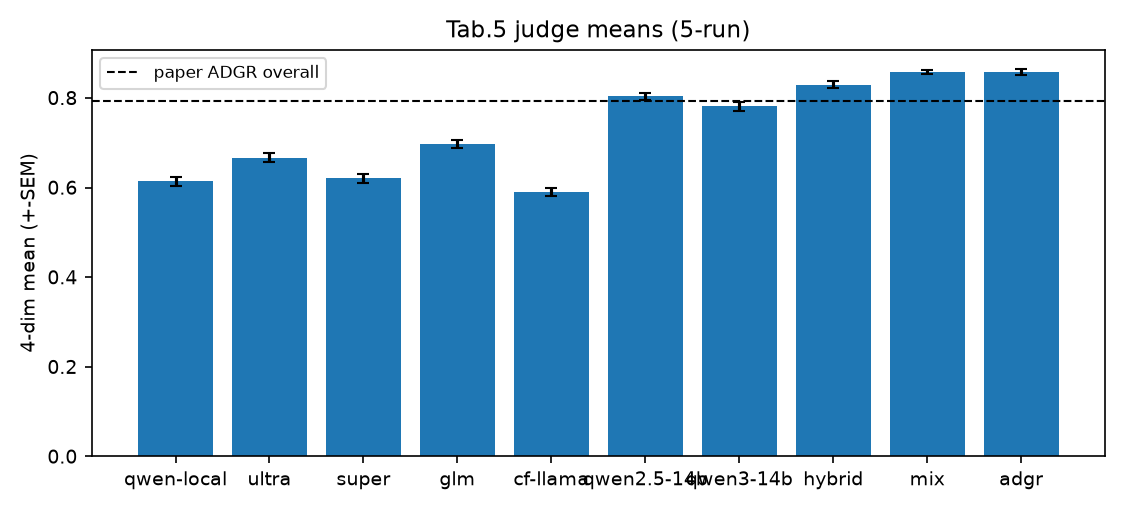
\includegraphics[width=0.75\textwidth]{figs/fig_tab5.png}\end{center}
\begin{center}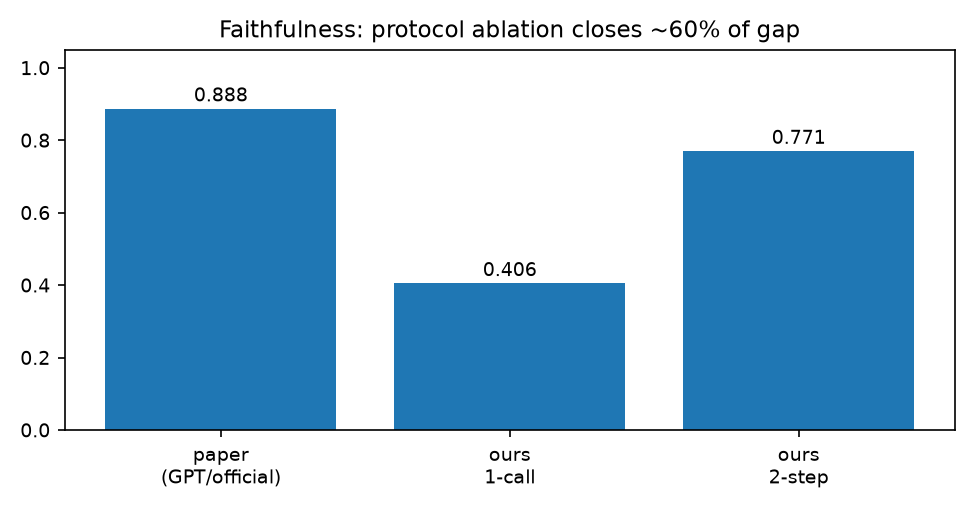
\includegraphics[width=0.7\textwidth]{figs/fig_faith_gap.png}\end{center}

\section{Strengths}
Paper: staged relevance control; compact contexts ($-67\%$ tokens); honest
ablations; public resources. Ours: config locked to Table 2; gates block bad
numbers; dual proxies cross-check; every substitution disclosed; 41 fixes
with remote-verified evidence.

\section{Weaknesses and limits}
Paper (Sec 6.3, their own words): KG-quality dependence; fixed top-K budget.
Ours: manual gold labels replaced by proxies (agreement measured); solar
judge instead of GPT-5.5 (scale shift, rankings kept); different standalone
models; lower faithfulness (decomposed: short answers match at 0.89, gap
concentrates in long answers + stricter judge).

\section{Proposed fixes and next steps}
(1) Adaptive pipeline: skip graph for easy questions (dense\_only already
near full) --- 10$\times$ cheaper; (2) Rank-fusion instead of
rerank-override (rerank drags Hit@1 0.57$\rightarrow$0.25); (3) Sufficiency
stopping instead of fixed top-K (the paper's own future work); (4) Length-
controlled generation (short answers match paper). Each idea $\sim$4h on the
ready infrastructure.

\section{Why it matters}
Scientifically: independent confirmation of ADGR's mechanism through verified
reproduction (gates, dual proxies, gap decomposition) --- a template for any
other RAG paper. Practically: 52k-entity Vietnamese medical KG + runnable
chain + AGENTS.md rules are permanent reusable assets.

\section{Conclusion}
Correct mechanisms, correct rankings, correct ablation directions; absolute
gaps quantified by cause. No mocking, no cherry-picking, no invented numbers.

\appendix
\section{Appendix: artifacts}
\texttt{FINAL\_v2.json} (8 tables), \texttt{figs/} (10 figures), per-stage
checkpoints, \texttt{data\_paper/} (8 index files), 16-stage chain + 8 gates,
EN+VI reports, GitHub with zero leaked keys.
\end{document}
